\documentclass[final]{beamer}

% ====================
% Packages
% ====================

\usepackage[T1]{fontenc}
 \usepackage[utf8]{luainputenc}
\usepackage{lmodern}
\usepackage[size=custom, width=197,height=235, scale=1.2]{beamerposter}
\usetheme{gemini}
\usecolortheme{msu}
\usepackage{graphicx}
\usepackage{booktabs}
\usepackage{tikz}
\usepackage{pgfplots}
\pgfplotsset{compat=1.14}
\usepackage{anyfontsize}
\usepackage{setspace}

% ====================
% Lengths
% ====================

% If you have N columns, choose \sepwidth and \colwidth such that
% (N+1)*\sepwidth + N*\colwidth = \paperwidth
\newlength{\sepwidth}
\newlength{\colwidth}
\setlength{\sepwidth}{0.018\paperwidth}
\setlength{\colwidth}{0.23\paperwidth}

\newcommand{\separatorcolumn}{\begin{column}{\sepwidth}\end{column}}

% ====================
% Title
% ====================

\title{MINE: Mutual Information Neural Estimation - A Comprehensive Exploration}

\author{
        \textbf{Student: Li Ge}\\
        \textbf{Instructor: Prof. Wu Youlong}\\
        \textbf{EE142 Final Project, ShanghaiTech University}}

% ====================
% Footer (optional)
% ====================

\footercontent{
  \href{mailto:youremail@msu.edu}{lige2022@shanghaitech.edu.cn}}
% (can be left out to remove footer)

% ====================
% Logo (optional)
% ====================

% use this to include logos on the left and/or right side of the header:

% Right: funding agencies and other affilations 
%\logoright{\includegraphics[height=7cm]{logos/NSF.eps}}
% ====================
% Body
% ====================

\begin{document}


\begin{frame}[t]
\begin{columns}[t]
\separatorcolumn

\begin{column}{\colwidth}

\begin{block}{Research Status of MI}
        \heading{Importance of MI}
        In contrast to correlation, MI captures \textbf{non-linear} statistical dependencies between variables, and thus can act as a measure of true dependence. 
        \heading{Challenges}
        Hard to conduct exact computation.
        \heading{Existing common approaches}
        Non-parametric (binning, likelihood ratio, KDE, approximate gaussianity), which is \textbf{not linearly related to the dimension of data and sample size}, leading to hard computation for high dimension data and thus \textbf{not general-purpose}. Recent work uses a dual formulation to estimate MI (through f-divergences ,including the KL-divergence) by adversarial deep neural networks. 

\end{block}

\begin{block}{Main Ideas of MINE}

    \begin{itemize}
      \item Exploiting \textbf{dual optimization} to estimate divergences goes beyond the minimax objective as formalized in GANs, which is demonstrated in the paper.
      \item MINE is designed based on dual representations of the KL-divergence with this idea, so that the model can be used in mutual information estimation, maximization, and minimization and is not confined to situation that involves an adversarial game.

    \end{itemize}

\end{block}

\begin{block}{Contributions}

    \begin{enumerate}
      \item Introduce MINE, which is scalable, flexible, and completely trainable via back-prop, as well as provide a thorough theoretical analysis.
      \item Show that the utility of this estimator (based on dual optimization) \textbf{transcends the minimax objective} as formalized in GANs.
      \item \textbf{GAN applications}: apply MINE to palliate mode-dropping in GANs and to improve reconstructions and inference in Adversarially Learned Inference on large scale datasets.
      \item \textbf{Information Bottleneck application}: use MINE to apply the Information Bottleneck method in a continuous setting, and show that this approach \textbf{outperforms variational bottleneck methods.}

    \end{enumerate}

\end{block}
  
\begin{block}{Theoretical Background}

      \heading{Mutual information}
      Equivalent to the Kullback-Leibler (KL-) divergence between the joint $\mathbb P_{XZ}$, and the product of the marginals $\mathbb P_X\otimes\mathbb P_Z$:
      \begin{equation}
          I(X, Z) = D_{KL}(\mathbb{P}_{XZ} \| \mathbb{P}_X \otimes \mathbb{P}_Z)
      \end{equation}
      Intuition: the larger the divergence between the joint and the product of the marginals, the stronger the dependence between $X$ and $Z$.
      \heading{Dual representations of the KL-divergence} 
      -- Key technical, alternative way to estimate KL-divergence and then alternative way to estimate MI.
        \begin{itemize}
        \item \textbf{The Donsker-Varadhan representation}:
            \begin{equation}
                D_{KL}(\mathbb{P} \| \mathbb{Q}) = \sup_{T:\Omega\to\mathbb{R}} \mathbb{E}_\mathbb{P}[T] - \log(\mathbb{E}_\mathbb{Q}[e^T])
            \end{equation}
            \textit{where the supremum is taken over all functions $T$ such that the two expectations are finite (integrability constraints). }\\
            For $\mathcal F$ be any class of functions $T : \Omega \to R$ satisfying the integrability constraints of the theorem:
            \begin{equation}
                D_{KL}(\mathbb{P} \| \mathbb{Q}) \geq \sup_{T \in \mathcal{F}} \mathbb{E}_{\mathbb{P}}[T] - \log(\mathbb{E}_{\mathbb{Q}}[e^T])
            \end{equation}
        \item \textbf{The f-divergence representation}:
        \begin{equation}
            D_{KL}(\mathbb{P} \| \mathbb{Q}) \geq \sup_{T \in \mathcal{F}} \mathbb{E}_{\mathbb{P}}[T] - \mathbb{E}_{\mathbb{Q}}[e^{T-1}]
        \end{equation}
        \item \textbf{Comparison}: - Comparison: for a fixed $T$, the Donsker-Varadhan bound is stronger (larger). Since log function restrain the growth compared to linear function by applying $x > e\log(x)$.
        \end{itemize}

\end{block}

\begin{alertblock}{Main Method}

      \heading{Idea}
      Choose $\mathcal F$ to be the family of functions $T_{\theta} : \mathcal X \times \mathcal Z \to \mathbb R$ parametrized by a deep neural network with parameters $θ ∈ Θ$. We call this network the statistics network. Thus we derive the relation:
        \begin{equation}
            I(X;Z) \geq I_{\Theta}(X;Z)
        \end{equation}
        \textit{where $I_{\Theta}(X;Z)$ is the neural information measure defined by the Donsker-Varadhan representation as:}
        \begin{equation}
            I_\Theta(X, Z) = \sup_{\theta \in \Theta} \mathbb{E}_{\mathbb{P}_{XZ}}[T_\theta] - \log(\mathbb{E}_{\mathbb{P}_X \otimes \mathbb{P}_Z}[e^{T_\theta}])
        \end{equation}
        \begin{itemize}
            \item $\mathbb P_{XZ}$ - unknown, sampled from paired data.
            \item $\mathbb P_X \otimes \mathbb P_Z$ - unknown, sample from data, or by shuffling another sample in the joint distribution and then calculate it’s marginal probability.
        \end{itemize}
      \heading{Define MINE}
        \begin{equation}
            \widehat{I(X;Z)}_n = \sup_{\theta \in \Theta} \mathbb{E}_{\mathbb{P}^{(n)}_{XZ}}[T_\theta] - \log(\mathbb{E}_{\mathbb{P}^{(n)}_X \otimes \mathbb{P}^{(n)}_Z}[e^{T_\theta}])
        \end{equation}
        \textit{where $\mathcal F = \{T_θ\}_{θ∈Θ}$ is the set of functions parametrized by a neural network, and $\hat{\mathbb P^{(n)}}$ is the empirical distribution associated to $n$ i.i.d. samples given a distribution $\mathbb P$. Also sometimes we do not use log function directly in the loss function, since the gradient becomes extremely large when the marginal mean tends to 0. Alternatively we may use the reciprocal of EAM to approximate log function, meanwhile detach this term to avoid gradient calculation. However we still use log every time when calculating MI.}

        \heading{Correcting bias from the stochastic gradients}
            \textbf{Problem}: In a mini-batch setting, the SGD gradients of MINE are biased. (Possible) bias source: 
            \begin{itemize}
                \item Nonlinear transformations (such as $\log$) are sensitive to small sample noise.
                \item Mini-batch samples are insufficient to fully represent the true distribution.
                \item Other dependencies between samples introduce additional errors.
            \end{itemize}
            \textbf{Solution in paper} - exponential moving average (EMA): For extremely small or large errors (which we analyzed earlier regarding their effects on nonlinear functions), due to the weight ${(1-\alpha)}^k$, \textbf{long-term cumulative effects are exponentially diluted}, resulting in smoother gradient updates and more stable training.\\
            ~\\
            \textbf{I also came up with some new solutions, which will be demonstrated later.}

\end{alertblock}

\begin{block}{Theoretical Properties}

      \heading{CONSISTENCY}
      -- Divided into two problems:
        \begin{itemize}
            \item 
            An approximation problem: related to the size of the function family $\mathcal F$: is $\mid\mathcal F\mid$ large enough to approximate optimal function $T^*$? - indeed! By \textbf{Universal Approximation Theorems for neural networks}. - Lemma 1 (approximation). (Also increase the hidden dimension of network to guarantee this!).\\
            \textbf{Lemma 1} (approximation). \textit{Let $\epsilon > 0$. There exists a neural network parametrizing functions $T_\theta$ with parameters $\theta$ in some compact domain $\Theta \subset \mathbb{R}^k$, such that}
            $$|I(X, Z) - I_\Theta(X, Z)| \leq \epsilon, \text{ a.e.}$$

            \item 
            An estimation problem: is estimated MI calculated from prior distribution (derived from sample results of two probabilities) approximate true MI with increasing sample size? - indeed! By classical consistency theorems for extremum estimators. - Lemma 2 (estimation).\\
            \textbf{Lemma 2} (estimation). \textit{Let $\epsilon > 0$. Given a family of neural network functions $T_\theta$ with parameters $\theta$ in some bounded domain $\Theta \subset \mathbb{R}^k$, there exists an $N \in \mathbb N$, such that}
            $$\forall n \geq N, |\widehat{I(X, Z)} - I_\Theta(X, Z)| \leq \epsilon, \text{ a.e.}$$

            \item Combining these two lemmas with the triangular inequality,  we have \textit{\textbf{MINE is strongly consistent.}}
        \end{itemize}
      \heading{SAMPLE COMPLEXITY}
            $$\tilde O(\frac{d\log d}{\epsilon^2})\text{, \textit{where $d$ is the dimension of the parameter space.}}$$

\end{block}

\begin{block}{Empirical Comparisons}

    This part is aimed to show that MINE has good performance when estimating MI and accounts for non-linear dependence.

      \heading{Comparing MINE to non-parametric estimation}
        \begin{itemize}
            \item Between MINE, MINE-$f$ and $k$-NN based non-parametric estimator.

            \item Consider multivariate Gaussian random variables: For multivariate Gaussian random variables $X_a$ and $X_b$, when the marginal distributions are standardized Gaussian distributions, their MI can be conveniently calculated by the correlation coefficient $\rho$:
            \begin{equation}
                 I(X_a; X_b) = -\frac{1}{2} \log(1 - \rho^2), \text{ where } |\rho| < 1.
            \end{equation}
            \item Results:
                \begin{figure}
                    \centering
                    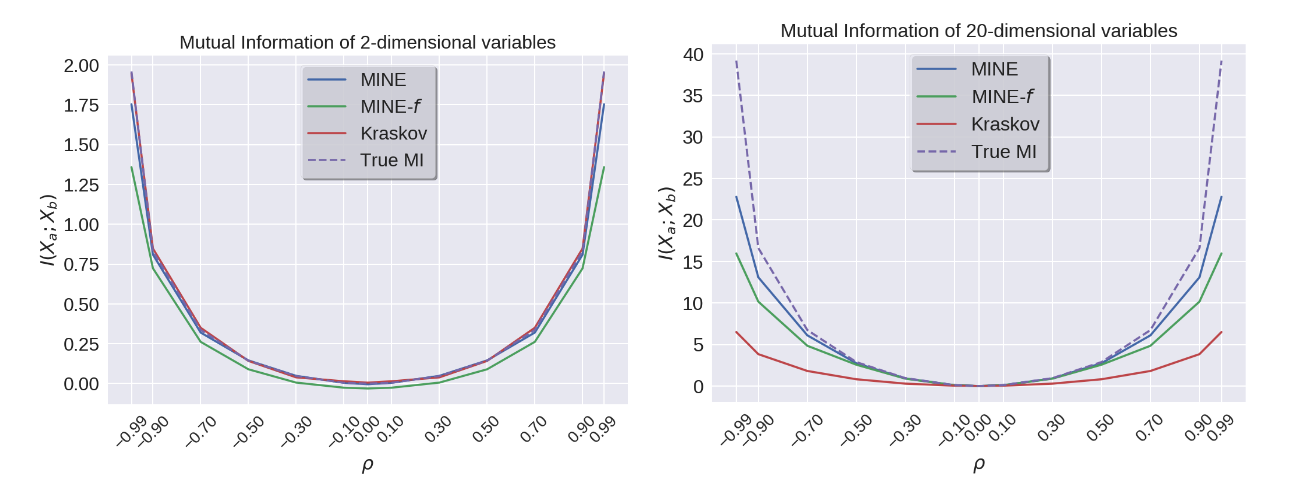
\includegraphics[width=0.95\textwidth]{figures/截屏2024-12-31 08.31.13.png}
                \end{figure}
        \end{itemize}
        
      \heading{Capturing non-linear dependencies}
        \begin{itemize}
            \item 
            \textbf{Equitability} - an important property of MI: For MI between random variables with relationship: $Y = f(X) + \sigma \odot \epsilon$, where $f$ is a deterministic non-linear transformation, $\epsilon$ is random noise, and $\sigma$ is a scalar representing the intensity of $\epsilon$, their MI depends only on the noise, $\sigma \odot \epsilon$.

            \item 
            Thus MINE is invariant to the choice of deterministic nonlinear transformation, consequently capturing non-linear statistical dependencies between variables.
        \end{itemize}

\end{block}

\end{column}
% ======================================================================================================
\separatorcolumn

\begin{column}{\colwidth}

\begin{block}{Applications}

    \begin{itemize}
      \item \textbf{MI maximization}: to improve \textbf{mode representation} and \textbf{reconstruction} of generative models.
      \item \textbf{MI minimization}: to effectively implement the information bottleneck in a continuous setting.
    \end{itemize}

\heading{Maximizing MI to improve GANs (mode coverage)}
$$\arg \max_G E[log(D(G([\epsilon, c])))] + βI(G([\epsilon, c]); c)$$
    \begin{table}[]
    \begin{tabular}{c c c}
    \toprule
    \textbf{Network} & \textbf{Input}            & \textbf{Input Meaning}                                    \\
    \midrule
    G               & $z$                       & Noise vector added to generator.                           \\
    D               & $(x ,  \tilde{x})$          & True samples and generated samples.                        \\
    MINE            & $(z ,  \tilde{x})$          & Noise vector and generated samples, in order to estimate $I(z ;\tilde{x})$. \\
    \bottomrule
    \end{tabular}
    \end{table}
\begin{itemize}
    \item Use adaptive gradient clipping: Since mutual information (MI) is theoretically unbounded, its gradient may differ significantly in magnitude compared to the gradient of the original loss component.
    

    \item Experiments: Spiral, 25-Gaussians datasets
    \begin{figure}
        \centering
        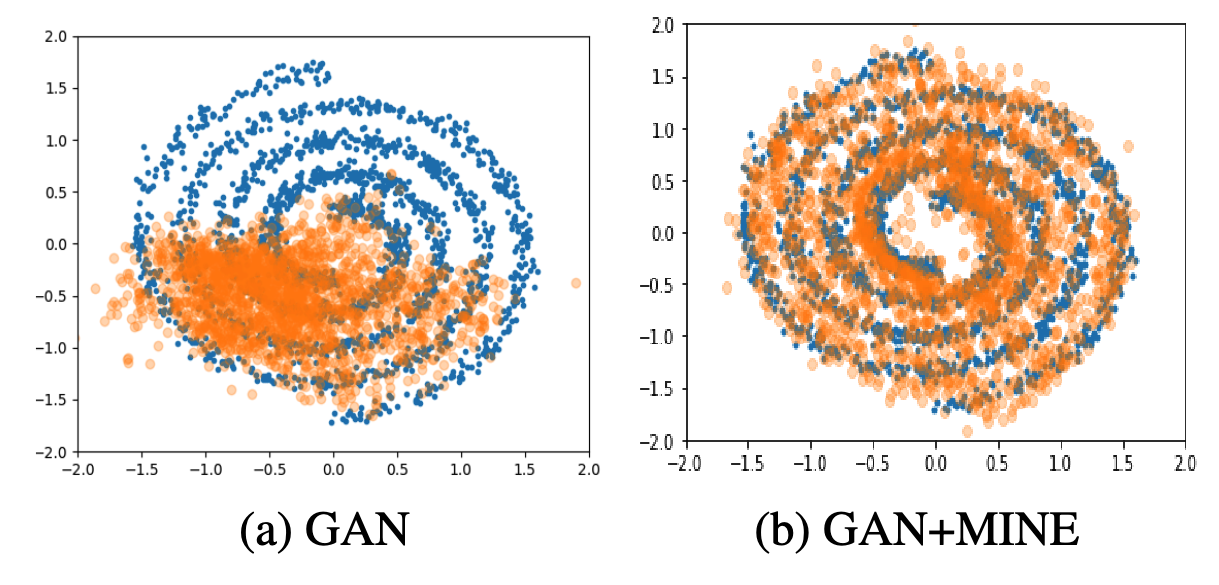
\includegraphics[width=0.75\linewidth]{figures/截屏2024-12-31 10.49.13.png}
    \end{figure}
    \begin{figure}
        \centering
        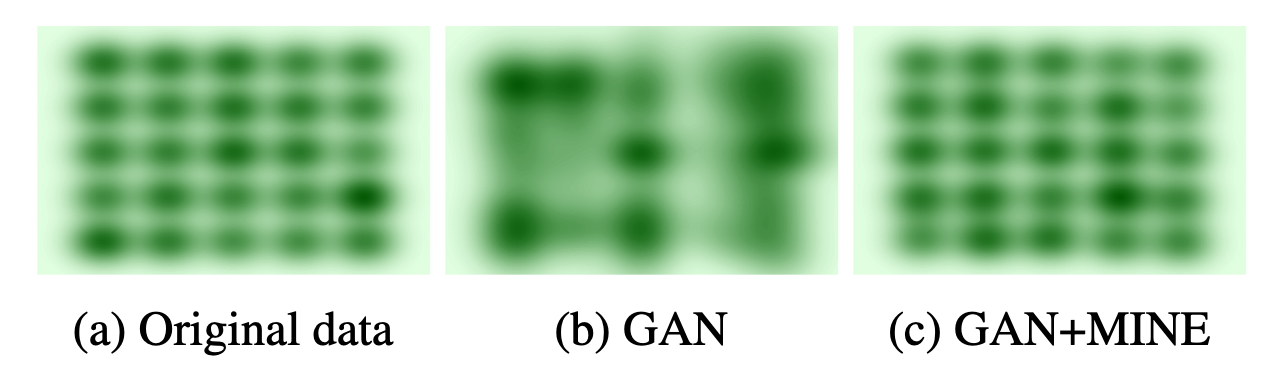
\includegraphics[width=0.95\linewidth]{figures/截屏2024-12-31 10.51.02.png}
    \end{figure}
    The results demonstrate that the MINE-based regularization significantly improves mode coverage in GANs.
    
    \item Experiment: Stacked MNIST (with 1000 unique modes)
    \begin{figure}
        \centering
        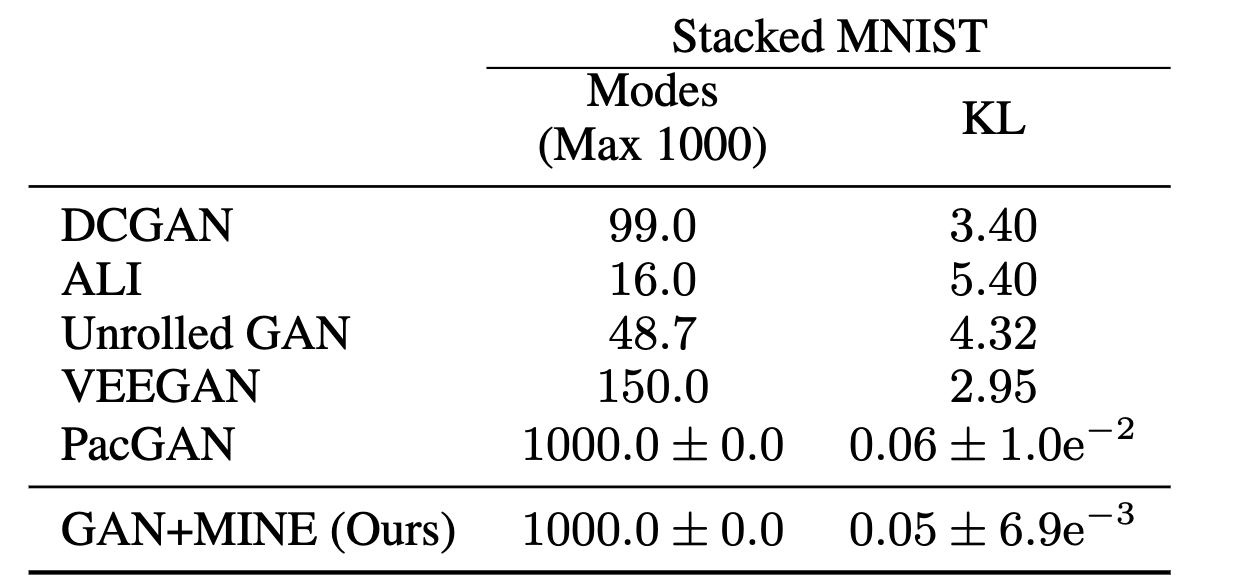
\includegraphics[width=0.7\linewidth]{figures/截屏2024-12-31 11.00.18.png}
    \end{figure}
    These results demonstrate that the MINE-based regularization enhances both the diversity (modes number) and accuracy (KL-divergence) of generated samples
    \begin{figure}
        \centering
        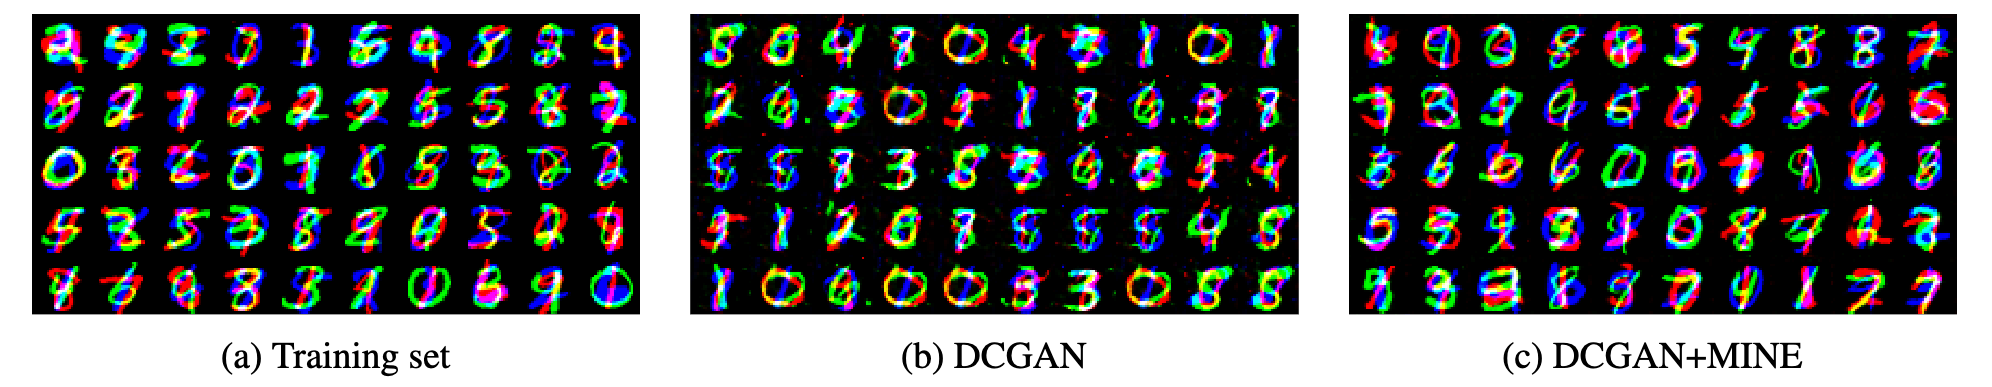
\includegraphics[width=1\linewidth]{截屏2024-12-31 11.01.56.png}
    \end{figure}
    
\end{itemize}

\heading{Maximizing MI to improve inference in bi-directional adversarial models (reconstruction)}
\begin{itemize}
    \item \textbf{Problem}: In practice ALI can lack fidelity (i.e., reconstructs less faithfully than desired), since for $X \to Z \to X^{\prime}$, the training objective of ALI is to make the joint distributions $q(x, z)$ and $p(x, z)$ match as closely as possible, without optimizing reconstruction error (difference between $X$ and $X^{\prime}$) directly and maximizing dependence between $X^{\prime}$ and $Z$:
    $$\min_G \min_F \max_D \mathbb{E}_{p(x, z)}[\log D(x, z)] + \mathbb{E}_{q(x, z)}[\log(1 - D(x, z))]$$

    \item \textbf{Improvement}: Since the reconstruction error can be bounded by:
    
    $$
    R \leq D_{KL}(q(x, z) || p(x, z)) - I_q(x, z) + H_q(z)
    $$
    
    we can minimize the reconstruction error by maximizing $I_q(x, z)$. Thus we can modify the training objective as:
    
    $$
    \arg \max_D \mathbb{E}_{q(x,z)}[\log D(x, z)] + \mathbb{E}_{p(x,z)}[\log (1 - D(x, z))]
    $$
    $$
    \arg \max_{F, G} \mathbb{E}_{q(x,z)}[\log (1 - D(x, z))] + \mathbb{E}_{p(x,z)}[\log D(x, z)] + \beta I_q(x, z)
    $$

    \item \textbf{Experiment: ALI+MINE}
    \begin{figure}
        \centering
        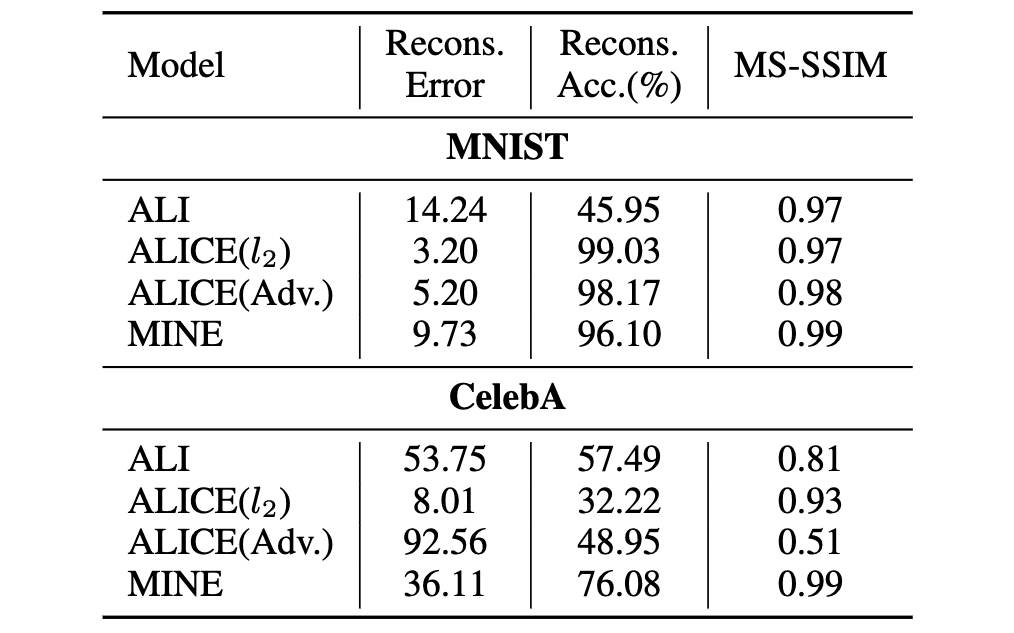
\includegraphics[width=0.75\linewidth]{figures/截屏2024-12-31 11.18.57.png}
    \end{figure}
    
    ALICE has slightly better performance than MINE in reconstruction, while the problem of mode-dropping (loss reconstruction accuracy) is much worse.
    
    \begin{figure}
        \centering
        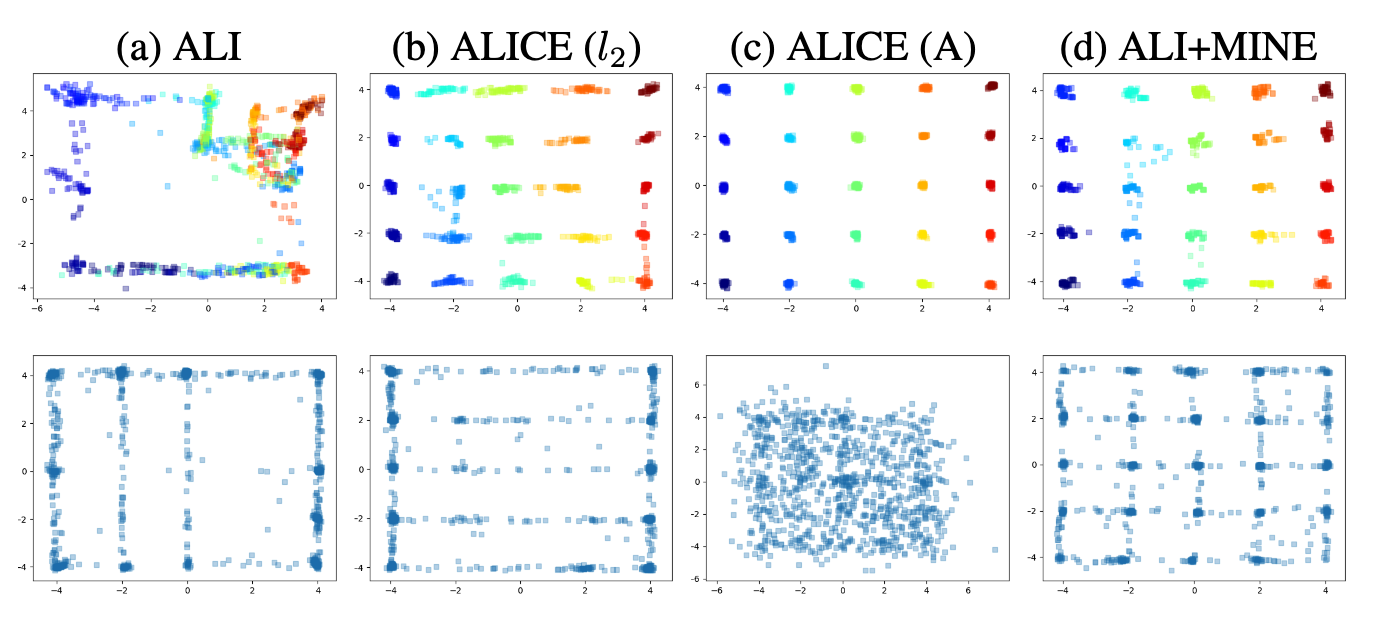
\includegraphics[width=0.95\linewidth]{截屏2024-12-31 11.20.38.png}
    \end{figure}
        
    
\end{itemize}


\heading{Information Bottleneck}
IB seeks an encoder, $q(Z \mid X)$, which includes Markovian structure $X \to Z \to Y$ by minimizing the loss function (IB Lagrangian): 
\begin{equation}
    \mathcal L[q(Z | X)] = H(Y | Z) + \beta I(X, Z)
\end{equation}
\begin{itemize}
    \item MINE can overcome the intractability of $I(X; Z)$ in the continuous setting of IB, and does not require a tractable density for the approximate posterior like variational bound methods.
    \item Related works includes discrete setting, jointly Gaussian continuous setting and variational bound.
    \item Experiment: Permutation-invariant MNIST classification\\
    - Define three types of encoders:\\
    1. A Gaussian encoder, same as DVB: $z = \mu(x) + \sigma \odot \epsilon, \quad \epsilon \sim \mathcal{N}(0, I)$.\\
    2. An additive noise encoder: $z = \text{enc}(x + \sigma \odot \epsilon), \quad \epsilon \sim \mathcal{N}(0, I)$.\\
    3. A propagated noise encoder: $z = \text{enc}([x, \epsilon]), \quad \epsilon \sim \mathcal{N}(0, I)$.\\
    \begin{figure}
        \centering
        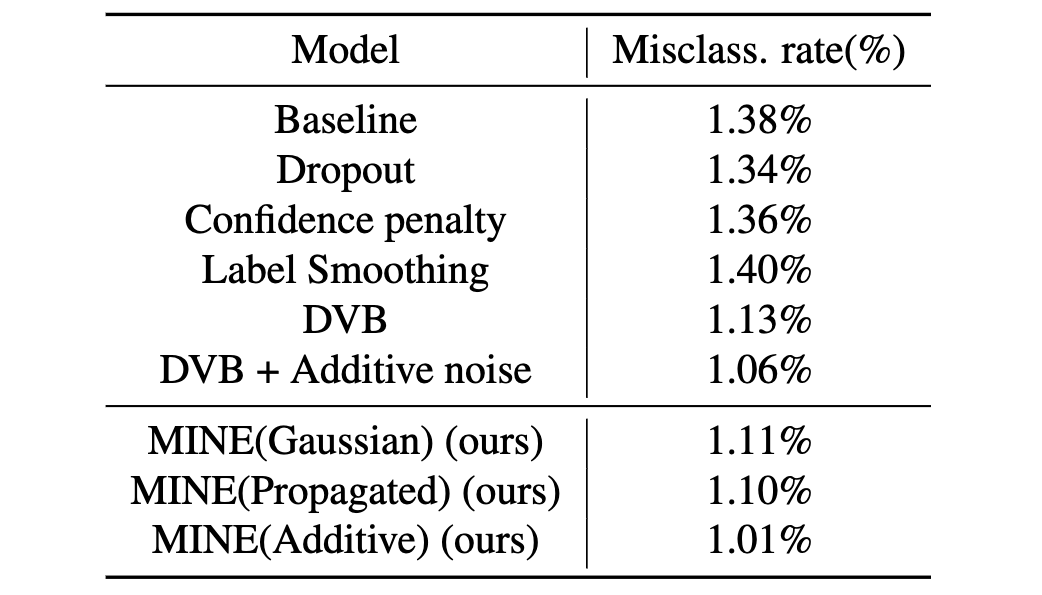
\includegraphics[width=0.75\linewidth]{figures/截屏2024-12-31 11.34.28.png}
    \end{figure}
    
\end{itemize}

\end{block}

\begin{block}{Conclusion}

    \begin{itemize}
      \item A term of MI can be introduced alleviate mode-dropping issue in GANs. 
      \item MI can also be used to improve inference and reconstructions in adversarially-learned inference. 
      \item MI allows for tractable application of Information bottleneck methods in a continuous setting.
    \end{itemize}

\end{block}

\end{column}
% ======================================================================================================
\separatorcolumn

\begin{column}{\colwidth}

  \begin{block}{Reproduction of the Paper on 3-D Gaussian}
    Dataset: Multivariate Gaussian Distributions with standardized normal marginal, since their MI can be conveniently calculated by the correlation coefficient $\rho$.\\
    ~\\
    Here I simply use the original loss function for MINE, which is (-MI):
    $$\mathcal L = - \left( \mathbb{E}_{P(X, Z)}[t] - \log \mathbb{E}_{P(X)P(Z)}\left[e^{t}\right] \right)$$
    \begin{figure}
    \centering
    \begin{minipage}{0.48\textwidth}
    \centering
    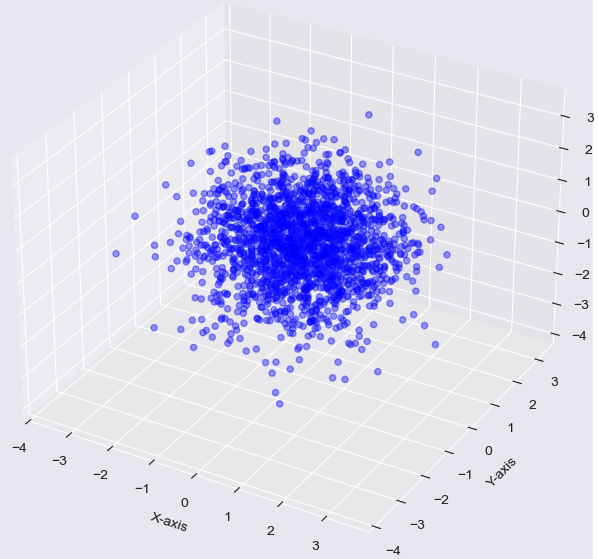
\includegraphics[width=0.9\linewidth]{截屏2024-12-31 12.07.47.png}
    \end{minipage}
    \begin{minipage}{0.5\textwidth}
    \centering
    \centering
    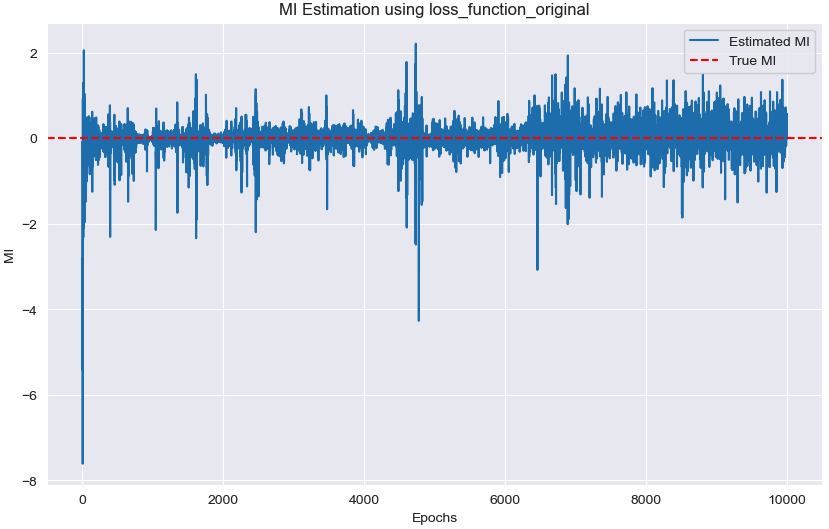
\includegraphics[width=0.9\linewidth]{figures/截屏2024-12-31 12.12.17.png}
    \end{minipage}
    \end{figure}
    Weakness - Numerical Instability: The term $\log \mathbb{E}[e^t]$ is highly sensitive to small variations in $t$, especially in small batch sizes. This can lead to large gradient fluctuations and potential instability during training.\\
  \end{block}

  \begin{block}{Improved Loss Function}
  \textbf{1. EAM loss function}:
  $$\mathcal L = - \left( \mathbb{E}_{P(X, Z)}[t] - \frac{1}{\mathbb{E}[\text{ma}(e^{t})]}\cdot \mathbb{E}_{P(X)P(Z)}\left[e^{t}\right] \right)$$
  Smoothing with Moving Average makes the optimization process smoother and reduces the sensitivity to the noise in the data.
  
  \textbf{2. Softplus loss function}:
  $$\mathcal{L} = - \left( \mathbb{E}_{P(X, Z)}[t] - \text{Softplus}\left(\mathbb{E}_{P(X)P(Z)}[e^t]\right) \right)$$
  A smoothed approximation of the $\max(x, 0)$ function. It avoids extreme values for very large or very small $t$, improving numerical stability.

  \textbf{3. Clipped gradient loss function}:
  $$\mathcal{L} = - \left( \mathbb{E}_{P(X, Z)}[t] - \log \mathbb{E}_{P(X)P(Z)}[e^t] \right)$$
  Weakness 1 - Gradient Distortion: Clipping modifies the true gradient direction, potentially leading to suboptimal convergence.\\
  Weakness 2 - Ineffectiveness for Directional Instability: While clipping addresses magnitude issues, it does not resolve directional instability caused by noisy or poorly scaled gradients.

  \textbf{4. Log-sum-exp loss function}:
  $$\mathcal{L} = - \left( \mathbb{E}_{P(X, Z)}[t] - \log \sum_{i} e^{t_i - \max(t)} \right)$$
  A standard technique for smoothing the gradient. \textbf{Specially}, it prevents numerical overflow or underflow, especially when computing sums of exponentials. \textbf{Also}, it constraints the sparse (like extremely small) data while still considering their contributions by considering the maximum.

  \textbf{5. Regularized loss function}:
  $$\mathcal{L} = - \left( \mathbb{E}_{P(X, Z)}[t] - \log \mathbb{E}_{P(X)P(Z)}[e^t] \right) + \lambda \|e^t\|_2^2$$
  Besides smoothing the gradient like other modified loss, it also prevents overfitting and thus improves the model's generalization.

  \textbf{6. Noise loss function}:
  $$\mathcal {L} = - \left( \mathbb{E}_{P(X, Z)}[t + \mathcal{N}(0, \sigma^2)] - \log \mathbb{E}_{P(X)P(Z)}[e^t] \right)$$
  Why add this?\\
  1. To improve the model’s robustness by encouraging it to learn more generalized representations.\\
  2. To encourage the model to explore different directions during optimization.\\
  Maybe the noise should be carefully chosen and combined with clipped gradient.

  \begin{figure}
    \centering
    \begin{minipage}{0.49\textwidth}
    \centering
    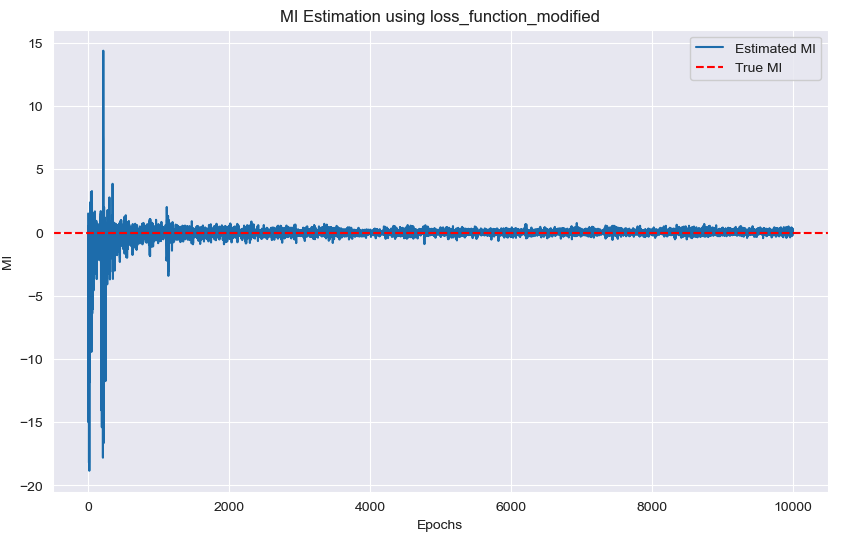
\includegraphics[width=1\linewidth]{MI_img/截屏2024-12-31 13.19.12.png}
    \end{minipage}
    \begin{minipage}{0.49\textwidth}
    \centering
    \centering
    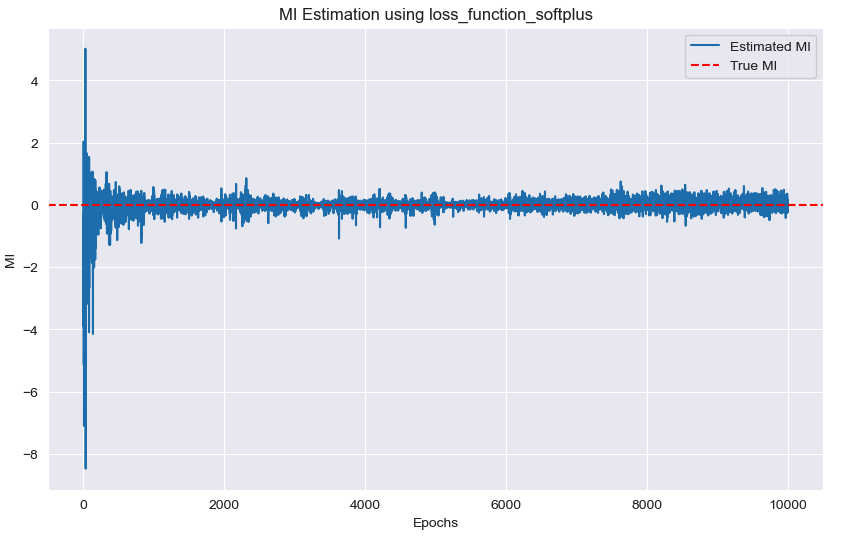
\includegraphics[width=1\linewidth]{MI_img/截屏2024-12-31 13.19.36.png}
    \end{minipage}
    \end{figure}

    \begin{figure}
    \centering
    \begin{minipage}{0.49\textwidth}
    \centering
    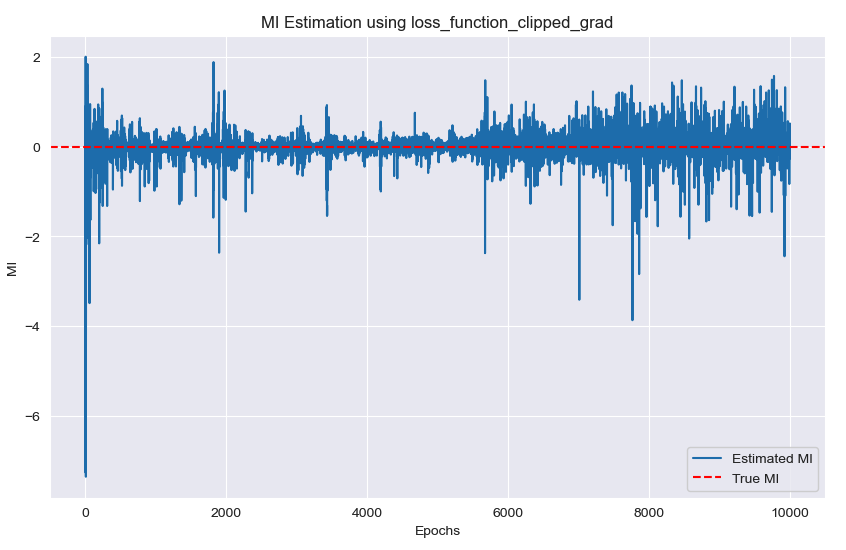
\includegraphics[width=1\linewidth]{MI_img/截屏2024-12-31 13.19.52.png}
    \end{minipage}
    \begin{minipage}{0.49\textwidth}
    \centering
    \centering
    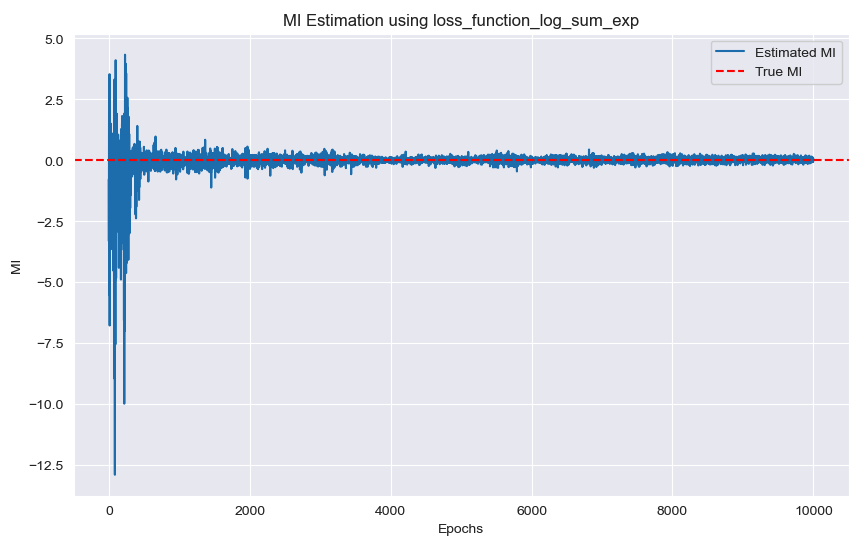
\includegraphics[width=1\linewidth]{MI_img/截屏2024-12-31 13.20.10.png}
    \end{minipage}
    \end{figure}

    \begin{figure}
    \centering
    \begin{minipage}{0.49\textwidth}
    \centering
    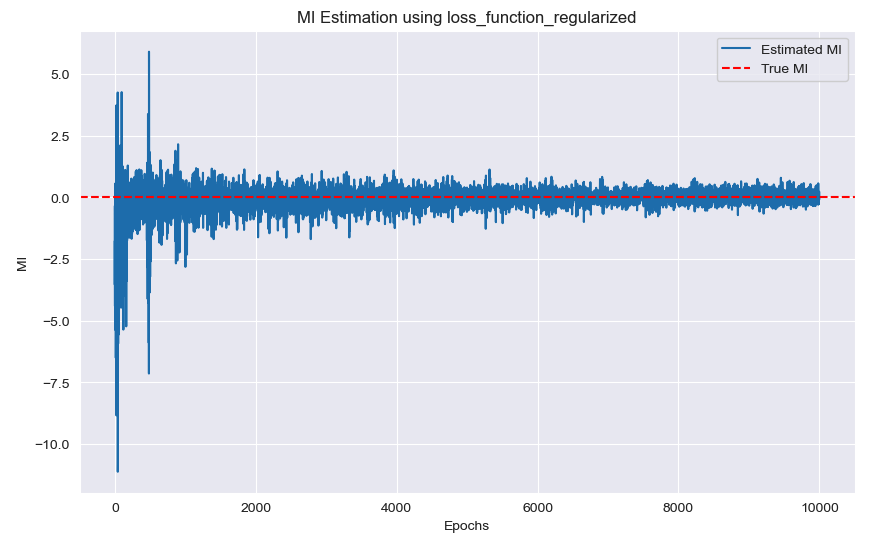
\includegraphics[width=1.05\linewidth]{MI_img/截屏2024-12-31 13.20.27.png}
    \end{minipage}
    \begin{minipage}{0.49\textwidth}
    \centering
    \centering
    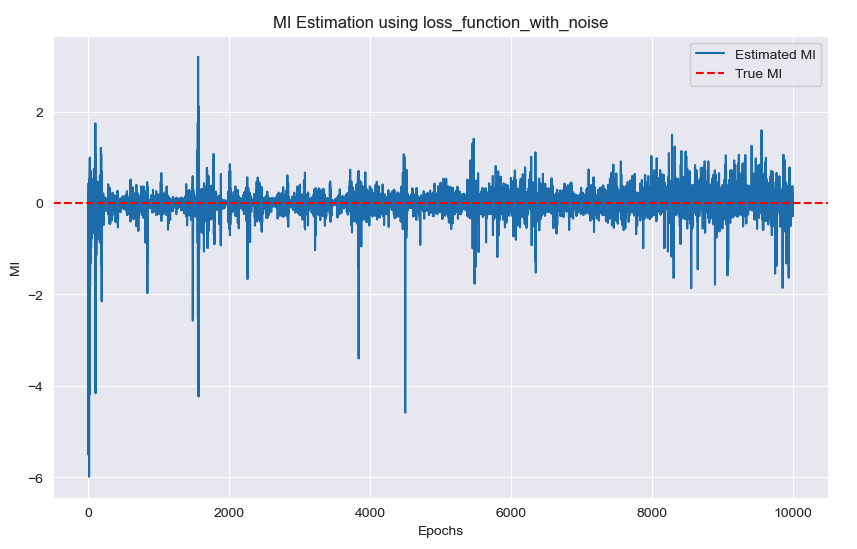
\includegraphics[width=1\linewidth]{MI_img/截屏2024-12-31 13.20.49.png}
    \end{minipage}
    \end{figure}

  \end{block}


  \begin{block}{Extra experiment on 4-D Gaussian}
    \begin{figure}
        \centering
        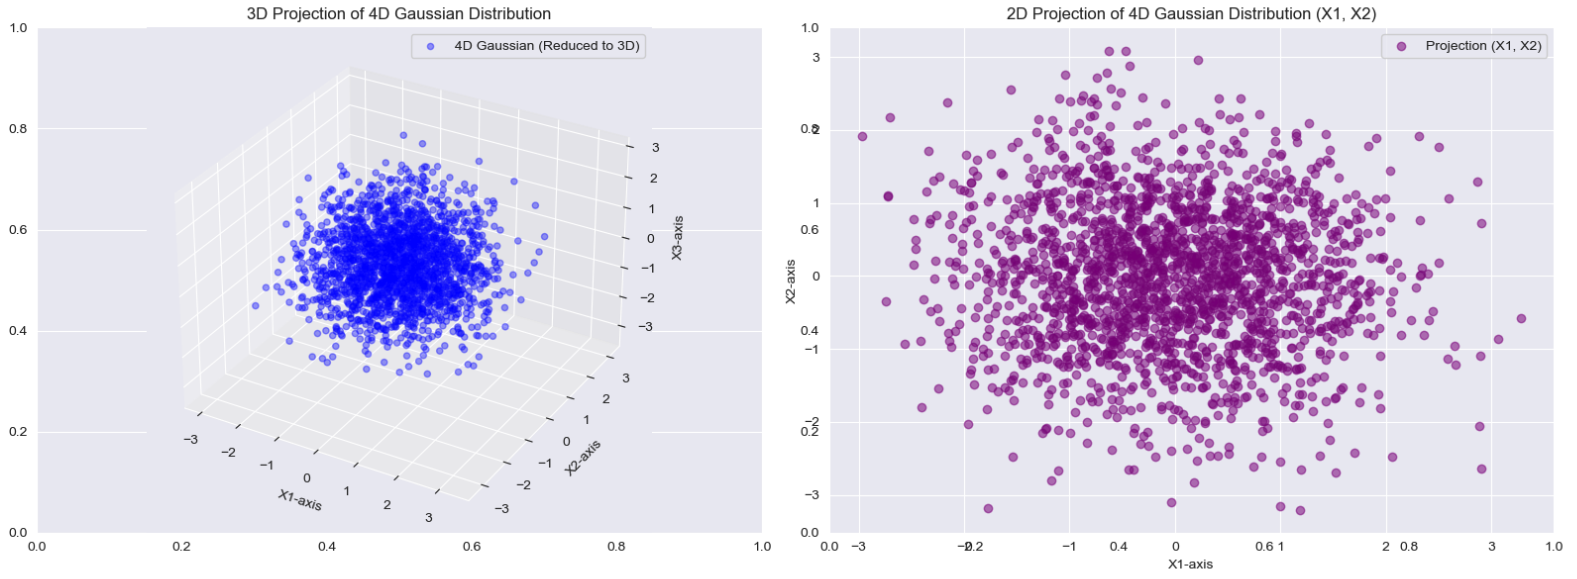
\includegraphics[width=1\linewidth]{截屏2024-12-31 13.43.13.png}
    \end{figure}

    \begin{figure}
      \centering
      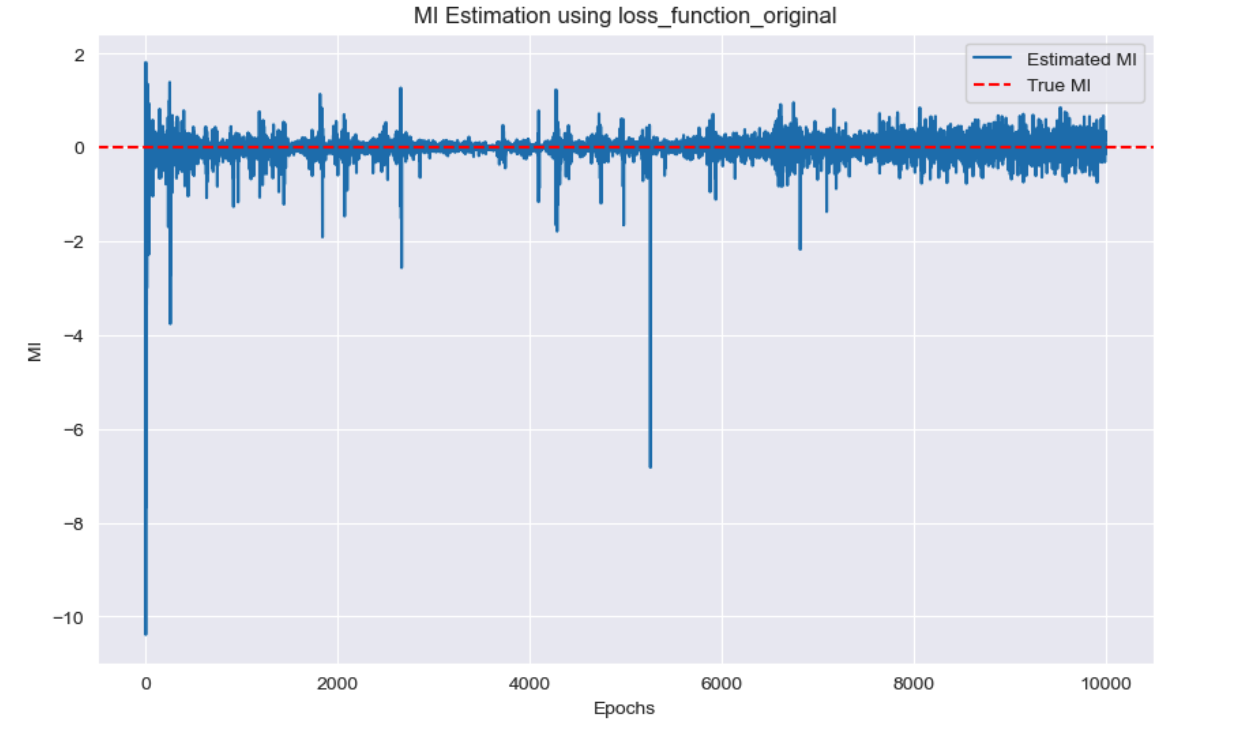
\includegraphics[width=0.52\linewidth]{截屏2024-12-31 13.55.00.png}
    \end{figure}

    \begin{figure}
    \centering
    \begin{minipage}{0.49\textwidth}
    \centering
    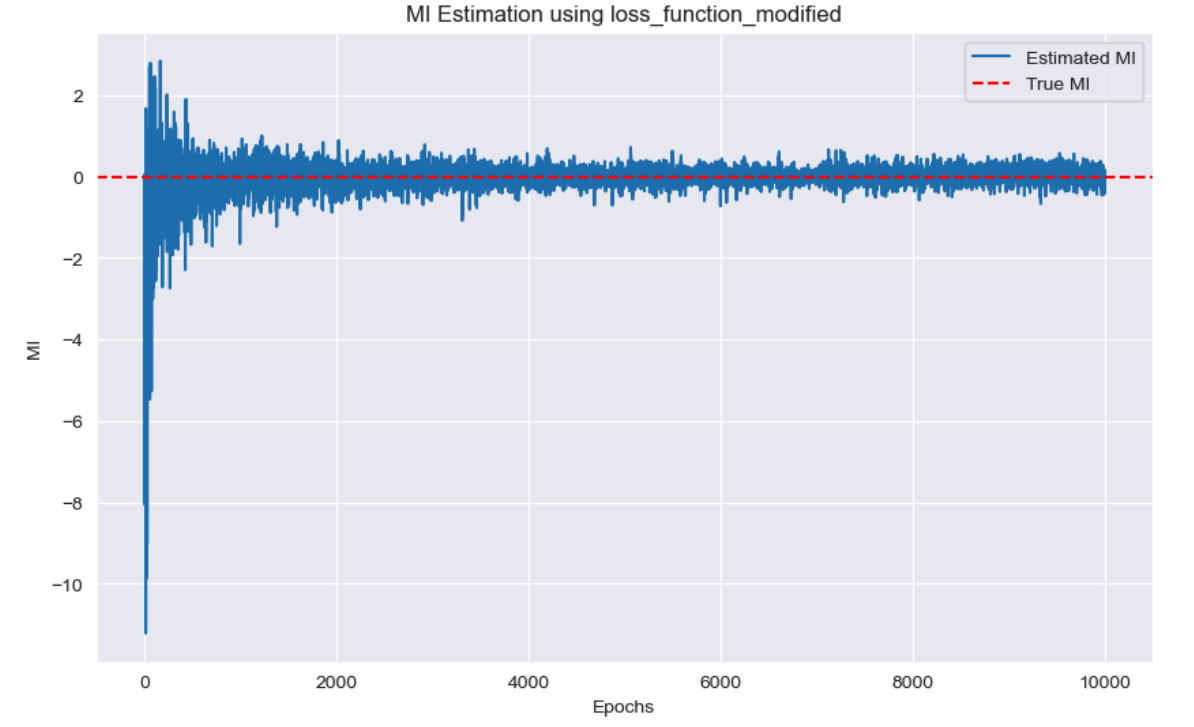
\includegraphics[width=1\linewidth]{4d/截屏2024-12-31 13.58.09.png}
    \end{minipage}
    \begin{minipage}{0.49\textwidth}
    \centering
    \centering
    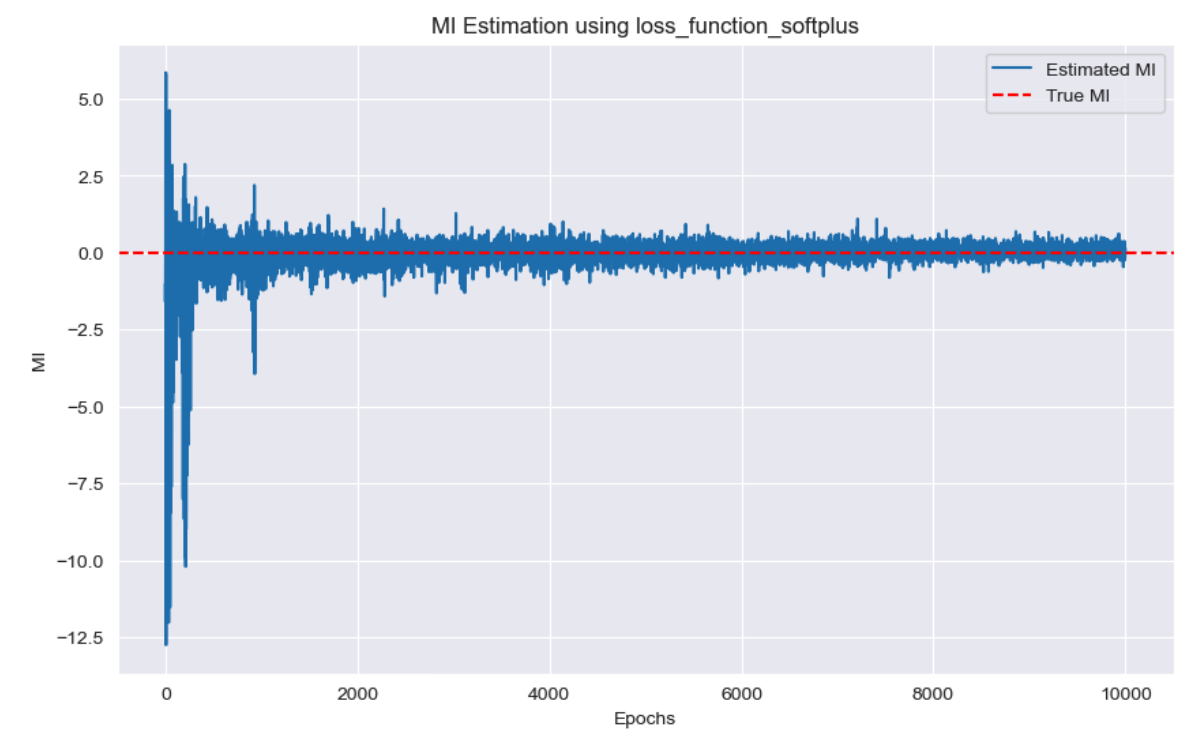
\includegraphics[width=1\linewidth]{4d/截屏2024-12-31 13.58.36.png}
    \end{minipage}
    \end{figure}

    \begin{figure}
    \centering
    \begin{minipage}{0.49\textwidth}
    \centering
    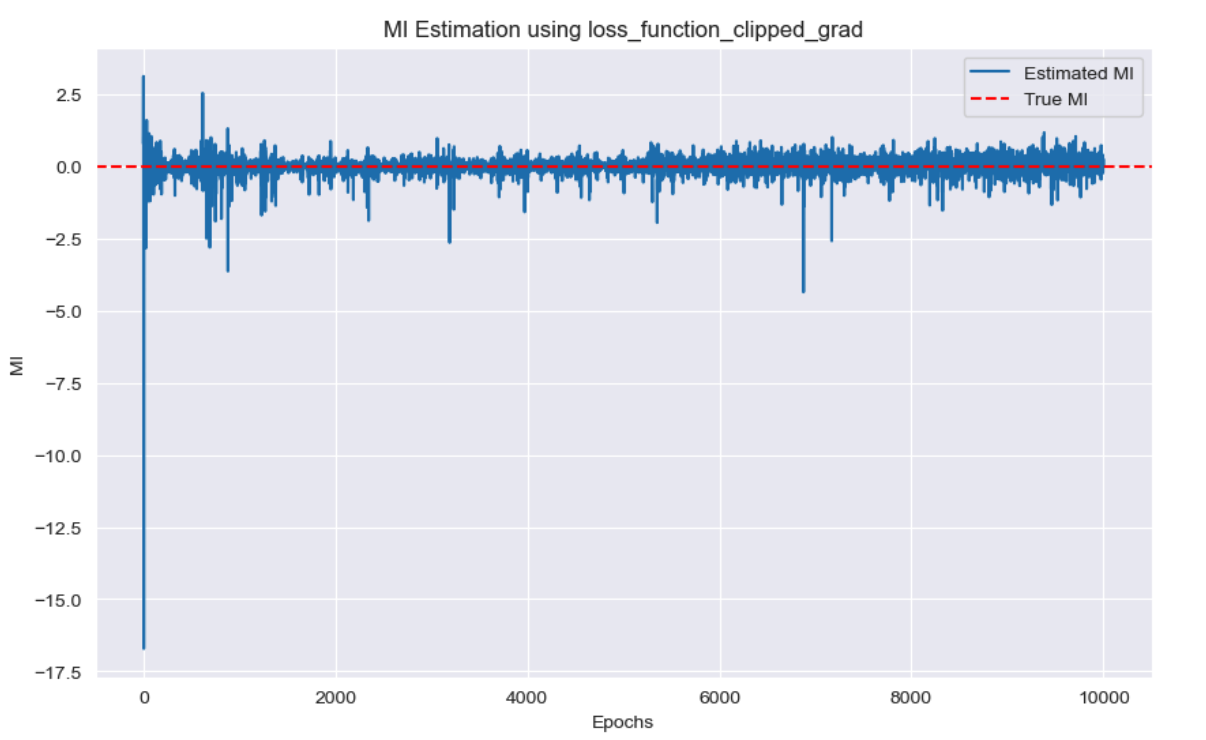
\includegraphics[width=1\linewidth]{4d/截屏2024-12-31 13.58.54.png}
    \end{minipage}
    \begin{minipage}{0.49\textwidth}
    \centering
    \centering
    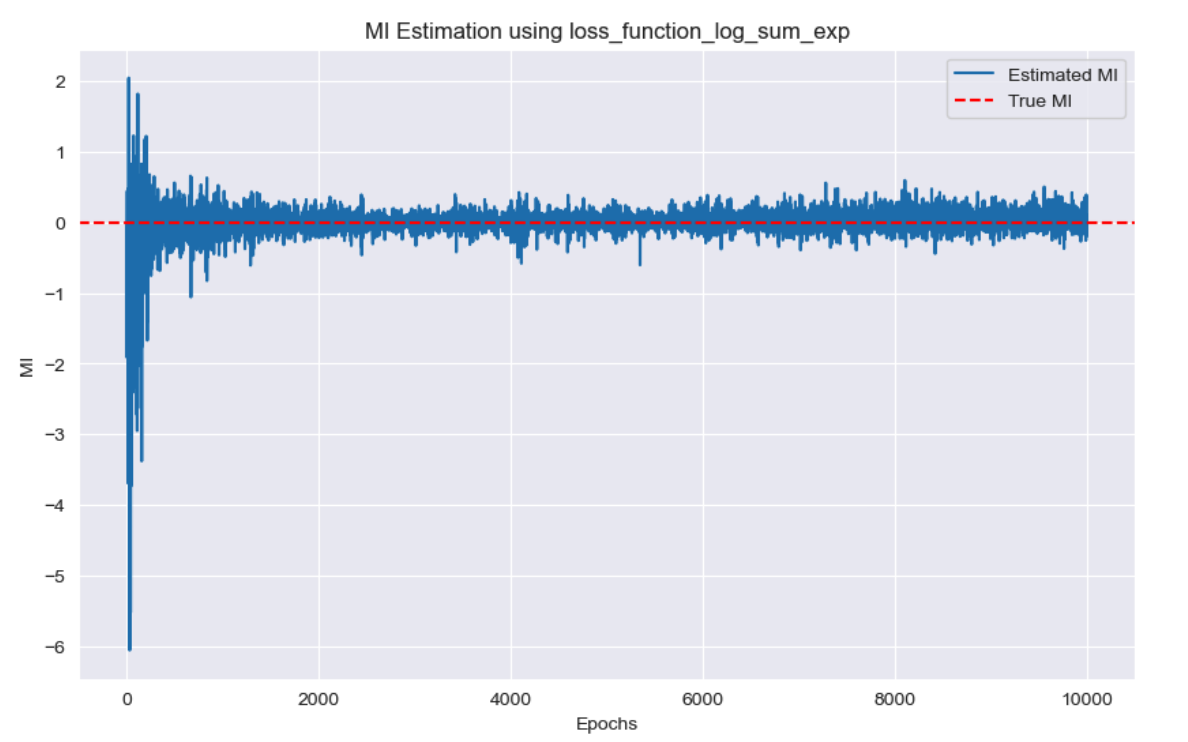
\includegraphics[width=1\linewidth]{4d/截屏2024-12-31 13.59.08.png}
    \end{minipage}
    \end{figure}

    \begin{figure}
    \centering
    \begin{minipage}{0.49\textwidth}
    \centering
    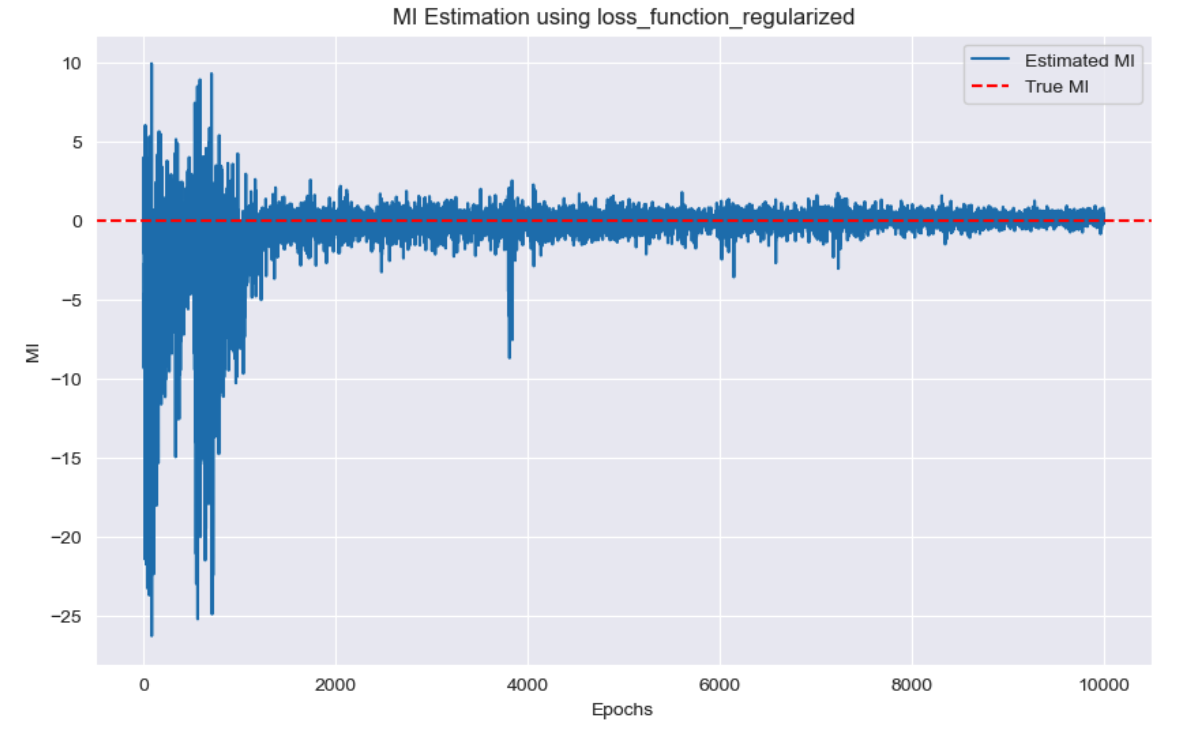
\includegraphics[width=1.02\linewidth]{4d/截屏2024-12-31 13.59.22.png}
    \end{minipage}
    \begin{minipage}{0.49\textwidth}
    \centering
    \centering
    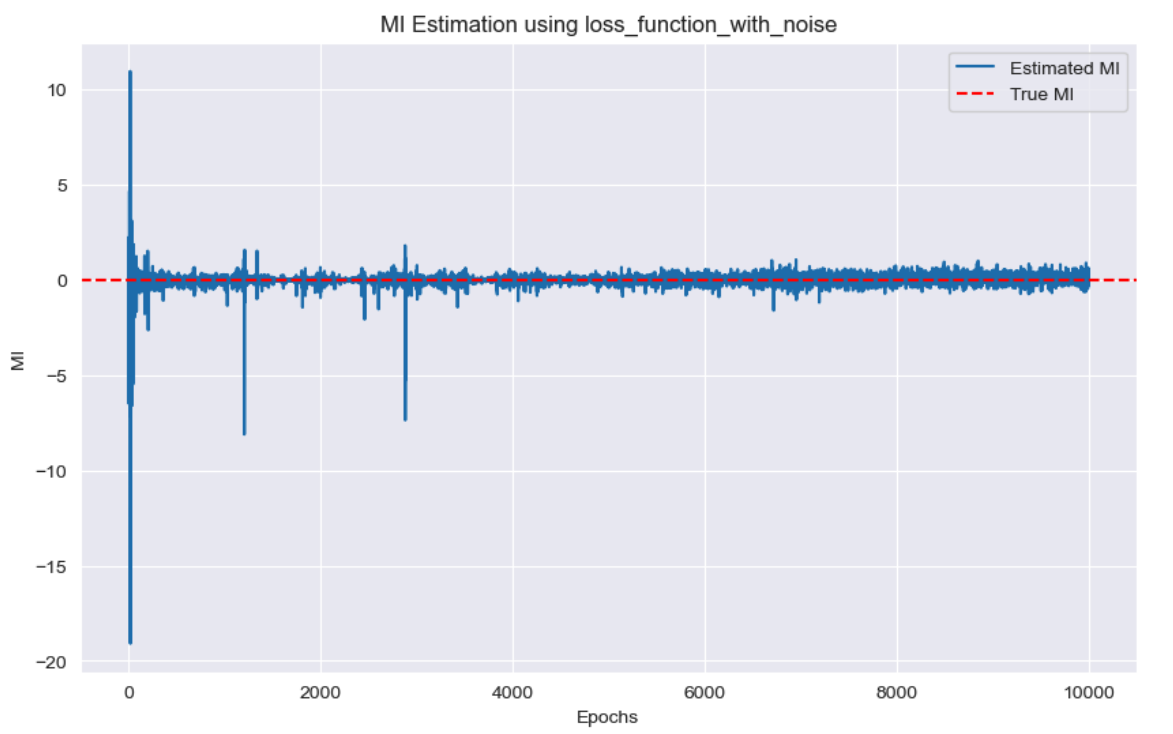
\includegraphics[width=1\linewidth]{4d/截屏2024-12-31 13.59.35.png}
    \end{minipage}
    \end{figure}
    
    \end{block}


\end{column}
% ======================================================================================================
\separatorcolumn

\begin{column}{\colwidth}


  \begin{block}{Experiments on GANs}
    \heading{Circle dataset}
    \begin{figure}
        \centering
        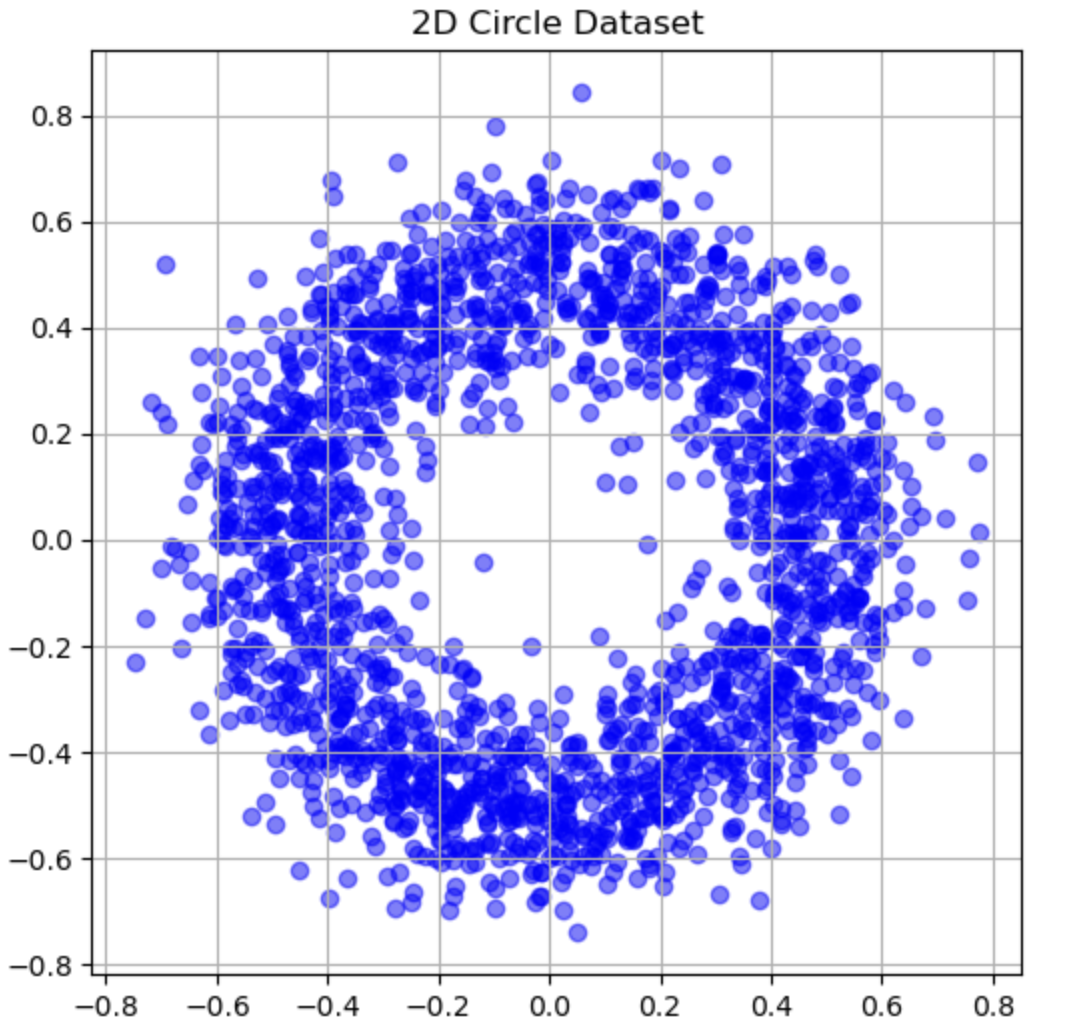
\includegraphics[width=0.3\linewidth]{截屏2024-12-31 23.56.23.png}
    \end{figure}

    \begin{figure}
    \centering
    \begin{minipage}{0.19\textwidth}
    \centering
    \includegraphics[width=1\linewidth]{gan_circle/Jietu20250101-000406@2x.png}
    \caption{$w=0$}
    \end{minipage}
    \begin{minipage}{0.19\textwidth}
    \centering
    \centering
    \includegraphics[width=1\linewidth]{gan_circle/Jietu20250101-000455@2x.png}
    \caption{$w=1$}
    \end{minipage}
    \begin{minipage}{0.19\textwidth}
    \centering
    \includegraphics[width=1\linewidth]{gan_circle/Jietu20250101-000526@2x.png}
    \caption{$w=0.1$}
    \end{minipage}
    \begin{minipage}{0.19\textwidth}
    \centering
    \includegraphics[width=1\linewidth]{gan_circle/Jietu20250101-000751@2x.png}
    \caption{$w=0.01$}
    \end{minipage}
    \begin{minipage}{0.19\textwidth}
    \centering
    \includegraphics[width=1\linewidth]{gan_circle/Jietu20250101-000818@2x.png}
    \caption{$w=0.001$}
    \end{minipage}
    \end{figure}


    \heading{Cross dataset}
    \begin{figure}
        \centering
        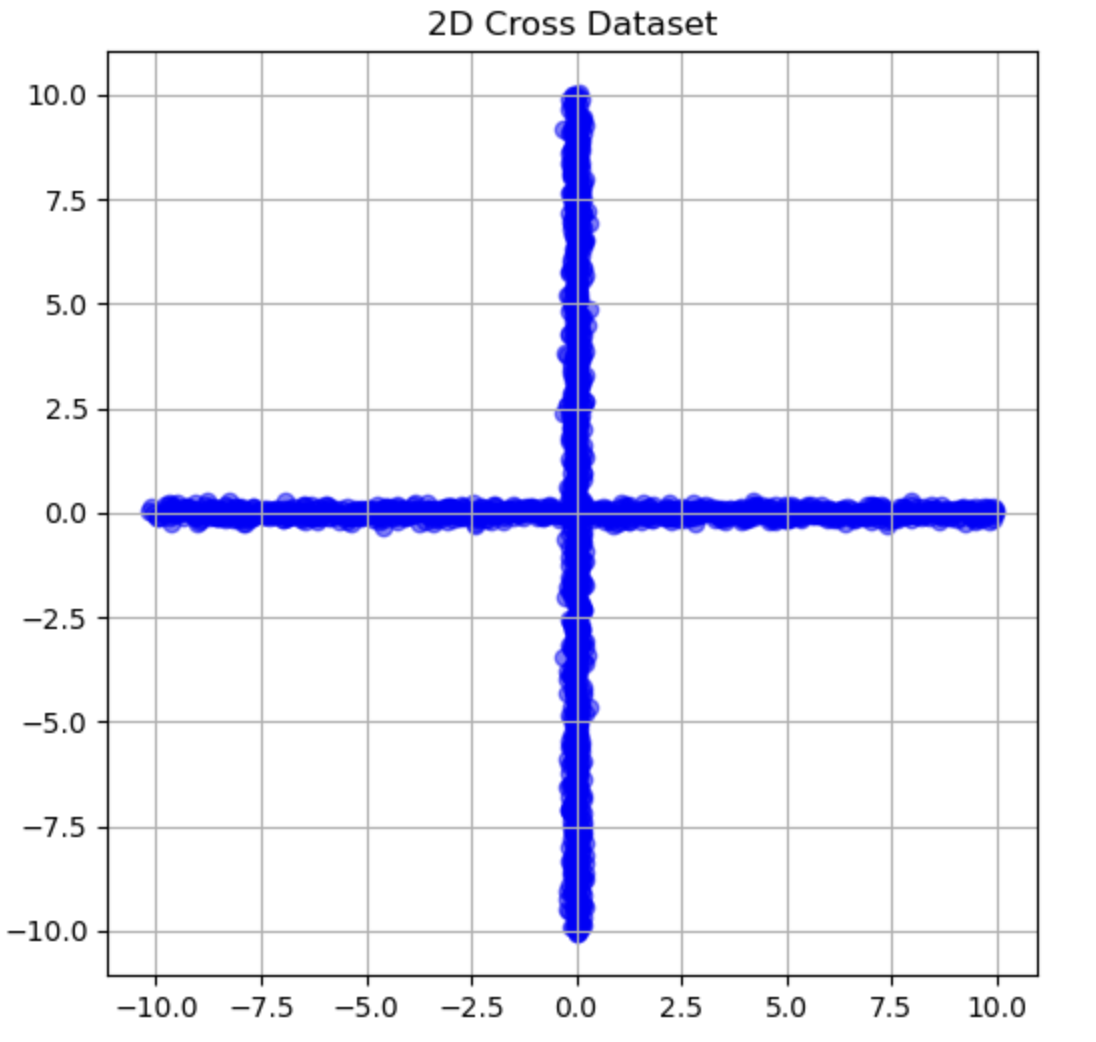
\includegraphics[width=0.3\linewidth]{截屏2025-01-01 00.28.52.png}
    \end{figure}

    \begin{figure}
    \centering
    \begin{minipage}{0.19\textwidth}
    \centering
    
\includegraphics[width=1\linewidth]{gan_cross/Jietu20250101-004224@2x.png}
    \caption{$w=0$}
    \end{minipage}
    \begin{minipage}{0.19\textwidth}
    \centering
    \centering
    
\includegraphics[width=1\linewidth]{gan_cross/Jietu20250101-004352@2x.png}
    \caption{$w=1$}
    \end{minipage}
    \begin{minipage}{0.19\textwidth}
    \centering
    
\includegraphics[width=1\linewidth]{gan_cross/Jietu20250101-003251@2x.png}
    \caption{$w=0.1$}
    \end{minipage}
    \begin{minipage}{0.19\textwidth}
    \centering
    
\includegraphics[width=1\linewidth]{gan_cross/Jietu20250101-003406@2x.png}
    \caption{$w=0.01$}
    \end{minipage}
    \begin{minipage}{0.19\textwidth}
    \centering
    
\includegraphics[width=1\linewidth]{gan_cross/Jietu20250101-003440@2x.png}
    \caption{$w=0.001$}
    \end{minipage}
    \end{figure}

    \begin{figure}
    \centering
    \begin{minipage}{0.49\textwidth}
        \centering
        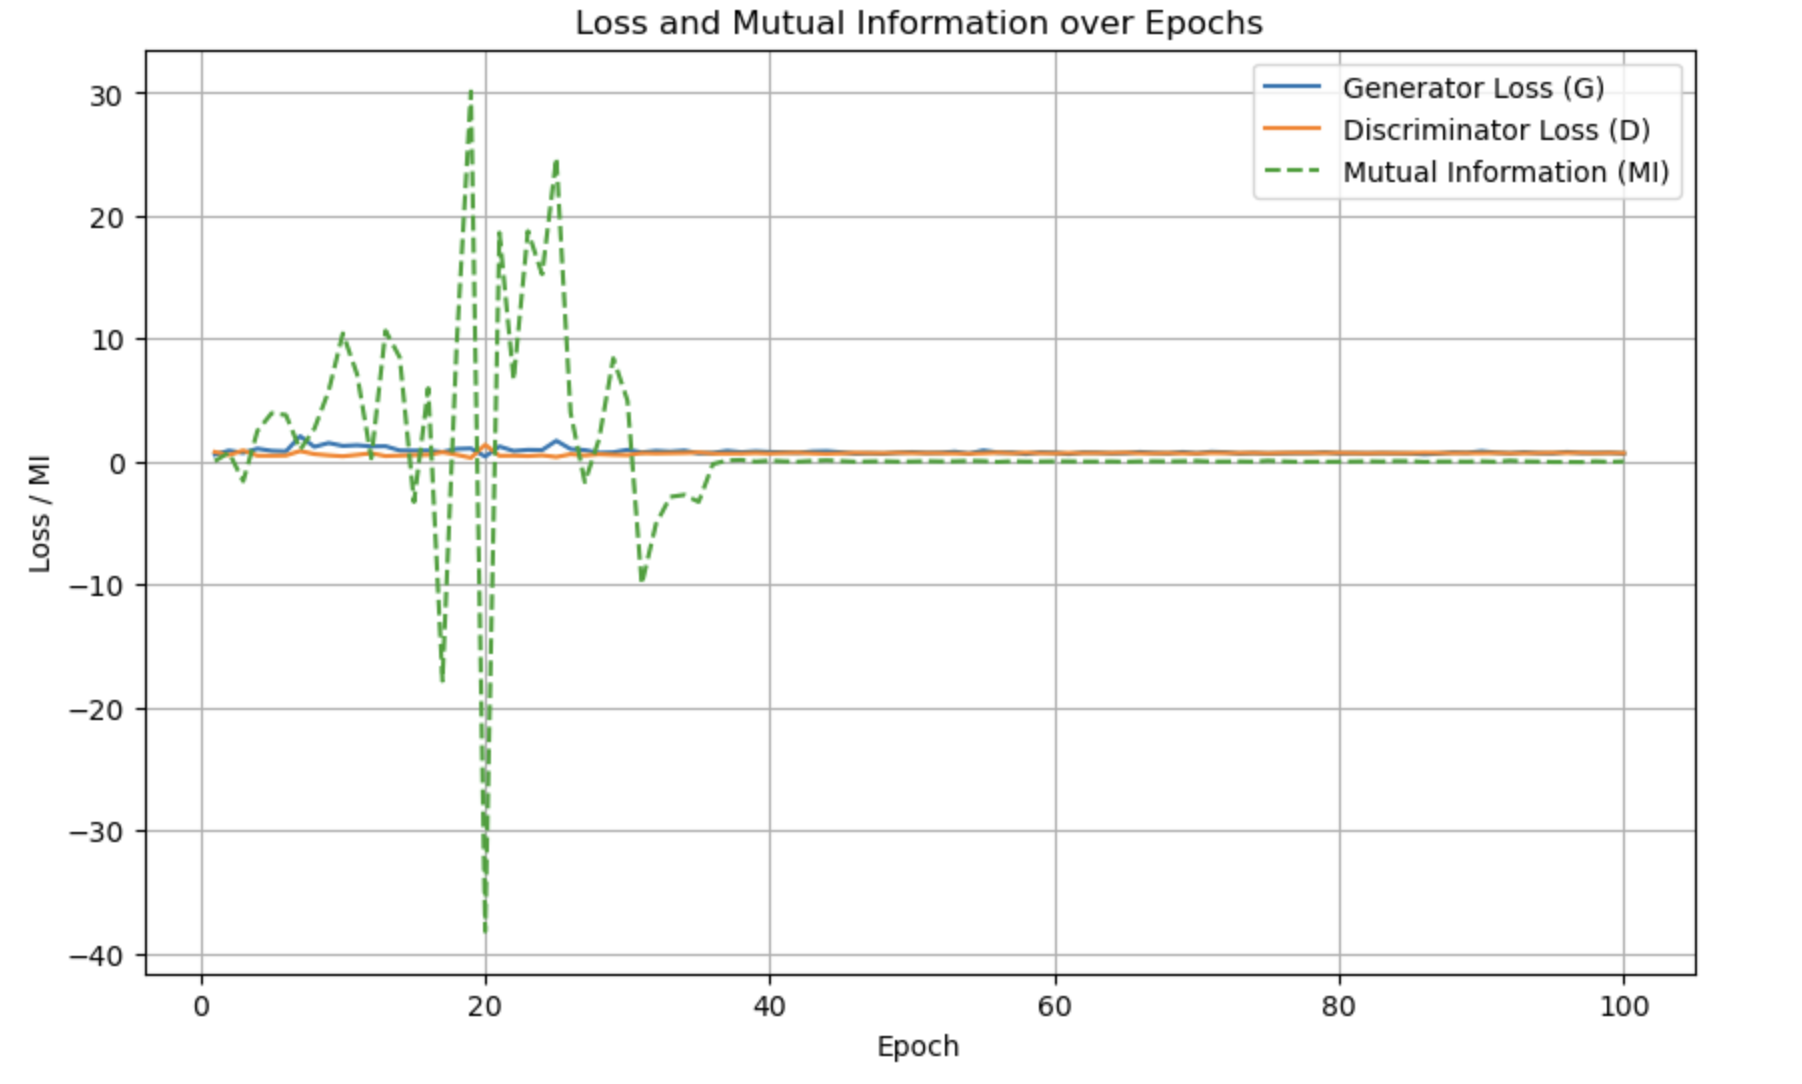
\includegraphics[width=1\linewidth]{截屏2025-01-01 00.47.33.png}
        \caption{$w=0$}
    \end{minipage}
    \begin{minipage}{0.49\textwidth}
        \centering
        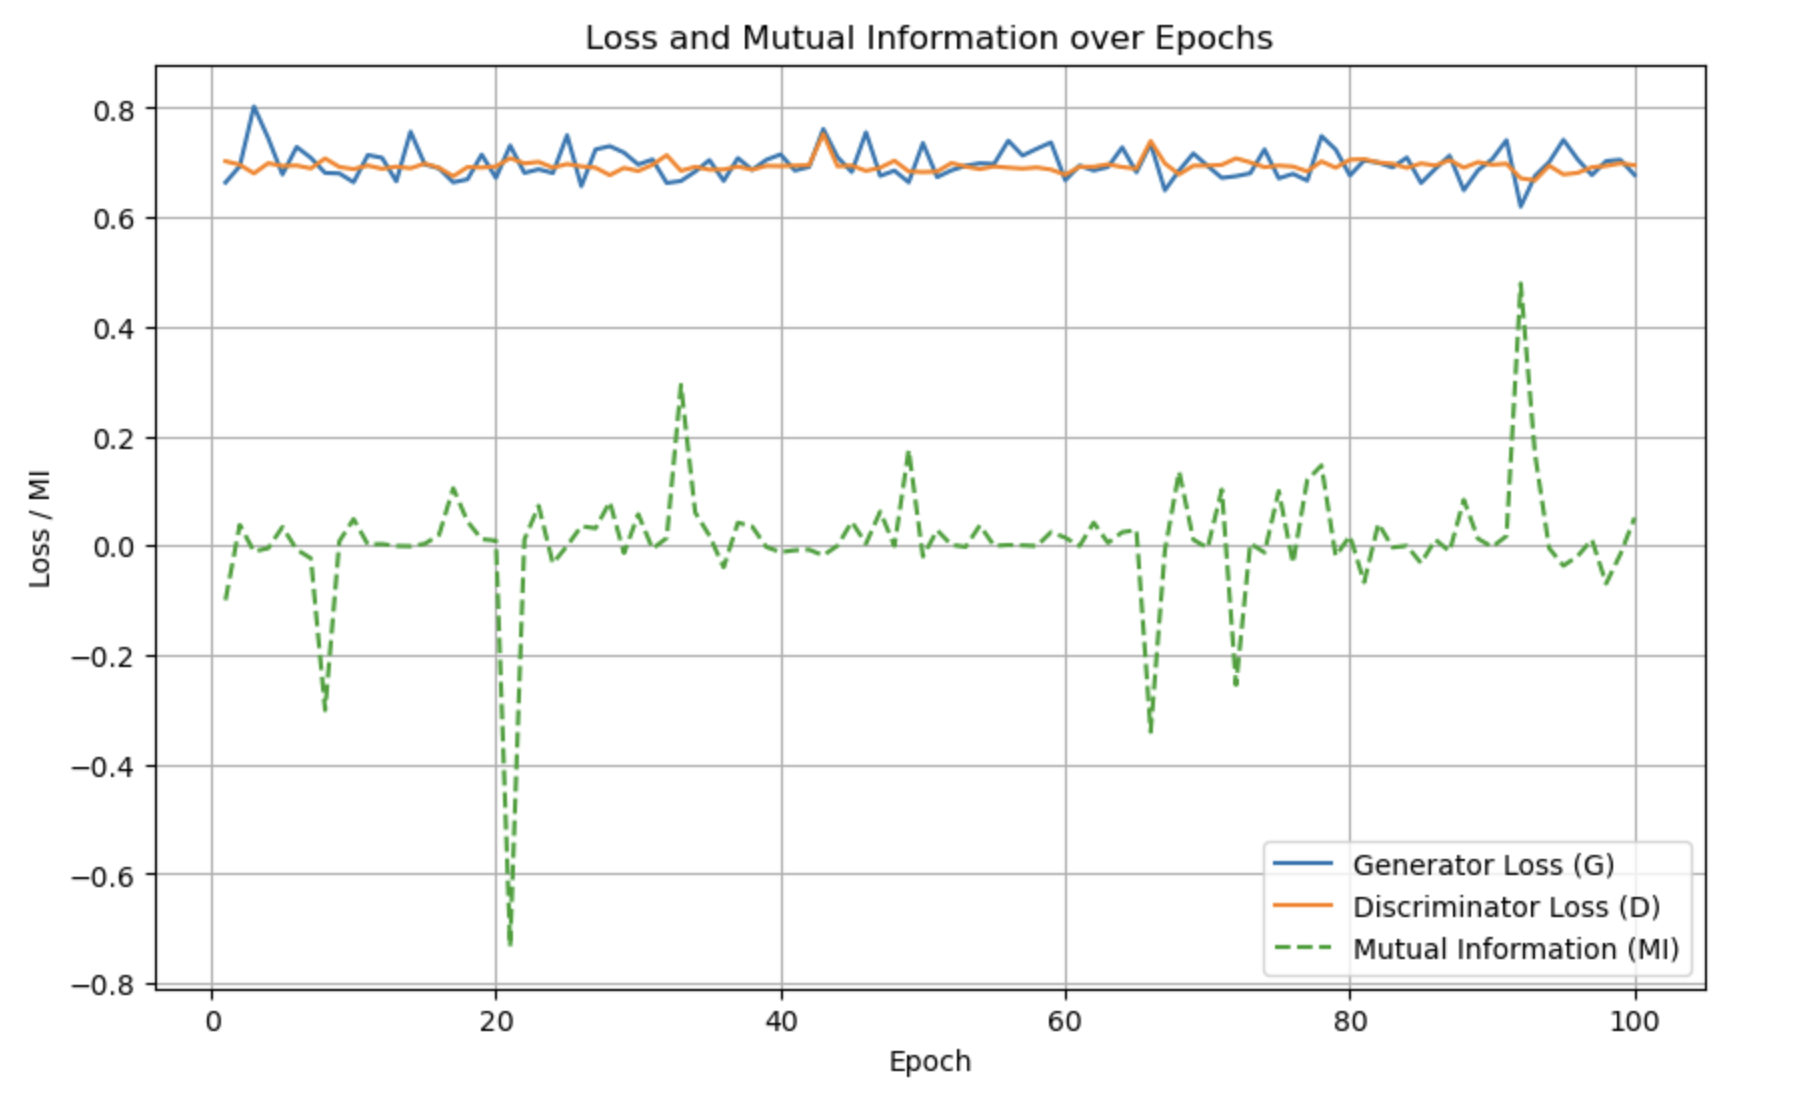
\includegraphics[width=1\linewidth]{截屏2025-01-01 00.47.09.png}
        \caption{$w=0.1$}
    \end{minipage}
    \end{figure}

    
        
  \end{block}

\end{column}

\separatorcolumn
\end{columns}
\end{frame}

\end{document}
